\subsection{Long-Slit Spectroscopy in L/M- and N-bands}

The purpose of the pipeline is to correct or remove contributions from
the instrument, telescope, and atmosphere and produce science-grade
data products for the L/M- and N-band long-slit spectroscopy
mode. Since the detector properties are not fully specified, especially of the new Geosnap, we currently assume
the same reduction cascade for both spectral ranges LM and
N. However, to keep flexibility and independence of both branches, we
define different recipes for the time being, although they will be
mostly based on the same algorithms. We therefore focus here on the LM-band only.

Figure~\ref{Fig:LMLssAssomap} shows the reduction cascade and the association map for the recipes handling L/M-long-slit
spectroscopy data.  Table~\ref{Tab:LssDatProc} contains the data processing table for this mode. For the time being it is not clear whether a geometric
distortion correction will be needed. We therefore consider to investigate
the geometry of atmospheric lines for this purpose. These lines also will
serve as reference frame for the wavelength calibration.

\begin{sidewaysfigure}[ht]
  \centering
  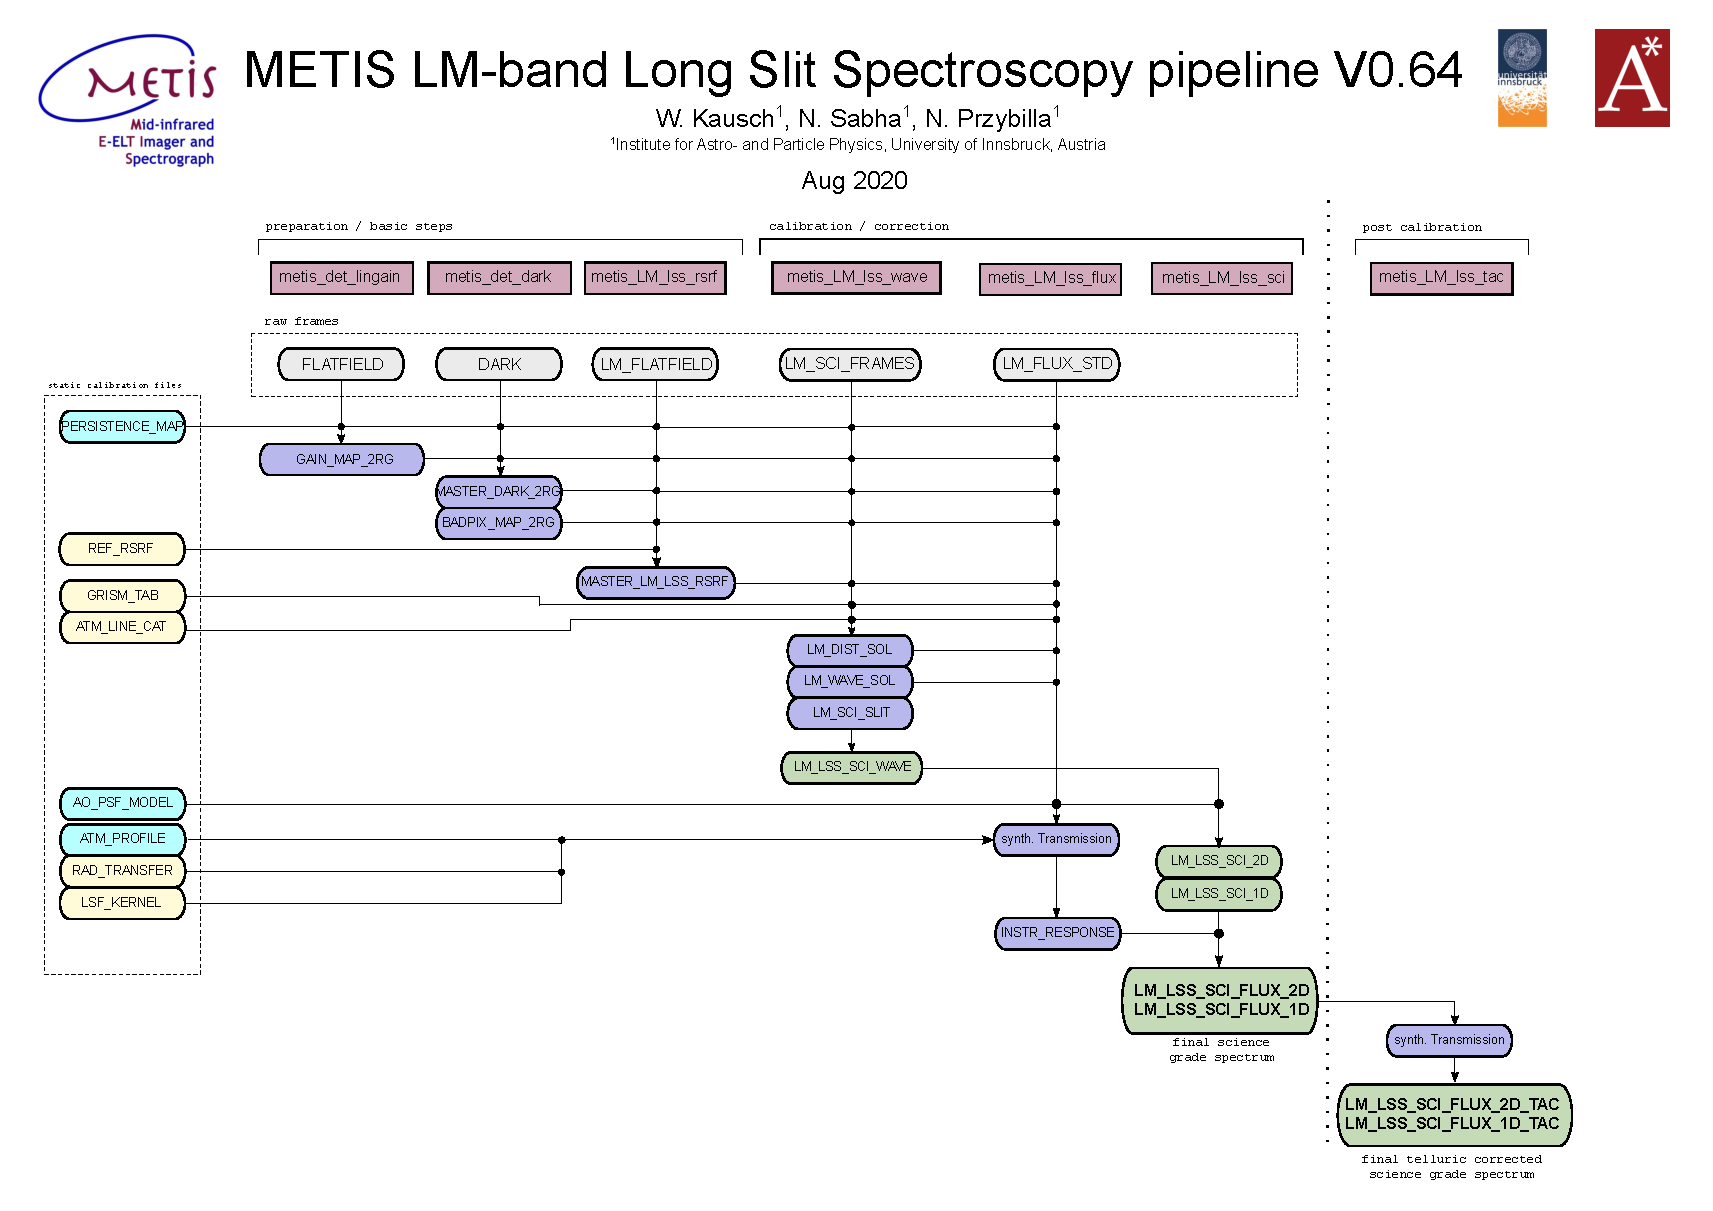
\includegraphics[width=0.9\textheight]{figures/LM_LSS_pipeline_wf_draft_latest_v0.64.pdf}
  \caption[Reduction cascade and association map for LM long-slit
  spectroscopy]{Reduction cascade and association map for long-slit
    spectroscopy in the LM bands.  }
  \label{Fig:LMLssAssomap}
\end{sidewaysfigure}

% \begin{sidewaysfigure}[ht]
%   \centering
%   \includegraphics[width=0.9\textheight]{figures/NQ_LSS_pipeline_wf_draft_latest.png}
%   \caption[Reduction cascade and association map for N long-slit
%   spectroscopy]{Reduction cascade and association map for long-slit
%     spectroscopy in the N band.  }
%   \label{Fig:NQLssAssomap}
% \end{sidewaysfigure}


%% ---- Table: LM long-slit spectroscopy
\begin{sidewaystable}
  \footnotesize
  \begin{center}
    \caption[Data Processing table for LM/N long-slit spectroscopy]{%
      Data Processing table for LM/N long-slit spectroscopy
      calibration modes}\bigskip
    \label{Tab:LssDatProc}
    \begin{tabular}{|l|l|l|l|l|l|}
      \hline
      Data Type   & Classification & Recipe (Level)	& FITS Keywords & CalibDB & Products\\
    (Templates) & Keywords	 & Processing steps	&		&	  &	\\
    \hline
    \TPL{DARK}	& \CODE{DPR.CATG==CALIB} & \REC{metis_det_dark} & Exposure time	&	& Averaged dark frame\\
    		& \CODE{DPR.TYPE==DARK}  &			&		&	& Bad pixel map\\
    		& \CODE{DPR.TECH==IMAGE}  &			&		&	& \\
    \hline
    \TPL{FLAT}	& \CODE{DPR.CATG==CALIB} & \REC{metis_LM_lss_rsrf} & Exposure time	& dark	& Averaged, normalized flatfield\\
    		& \CODE{DPR.TYPE==FLAT}  &			&		&	& Bad pixel map\\
    		& \CODE{DPR.TECH==SPECTRUM}  &			&		&	& \\
    \hline
    \TPL{SCIENCE} & \CODE{DPR.CATG==SCIENCE} & \REC{metis_LM_lss_wave} & Object name &  Line list & wavelength solution\\
    		& \CODE{DPR.TYPE==LSS}   &			   & Exposure time & &\\
    		& \CODE{DPR.TECH==SPECTRUM}  &			&		&	& \\
    		& \CODE{PRO.CATG==SPECTRUM}   &  &  & & \\
    \hline
    \TPL{SCIENCE} & \CODE{DPR.CATG==SCIENCE} & \REC{metis_LM_lss_sci} & Object name & 	 & Science grade spectrum\\
    		& \CODE{DPR.TYPE==LSS}   &			   & Exposure time & &\\
    		& \CODE{DPR.TECH==SPECTRUM}  &			&		&	& \\
    		& \CODE{PRO.CATG==SPECTRUM}   &  &  & & \\
    \hline
    \TPL{SCIENCE} & \CODE{DPR.CATG==SCIENCE} & \REC{metis_LM_lss_flux} & Object name (Flux STD) & reference flux of STD & Science grade, flux calibrated spectrum\\
    		& \CODE{DPR.TYPE==LSS}   &			   & Exposure time & &\\
    		& \CODE{DPR.TECH==SPECTRUM}  &			&		&	& \\
    		& \CODE{PRO.CATG==SPECTRUM}   &  &  & & \\
    \hline
    \TPL{SCIENCE} & \CODE{DPR.CATG==SCIENCE} & \REC{metis_LM_lss_tac} & Object name & 	 & Science grade telluric\\
    		& \CODE{DPR.TYPE==LSS}   &			   & Transmission curve & &Absorption corrected spectrum\\
    		& \CODE{DPR.TECH==SPECTRUM}  &			&		&	& \\
    		& \CODE{PRO.CATG==SPECTRUM}   &  &  & & \\
    \hline
    \end{tabular}
  \end{center}
\end{sidewaystable}

\begin{figure}[ht]
  \centering
  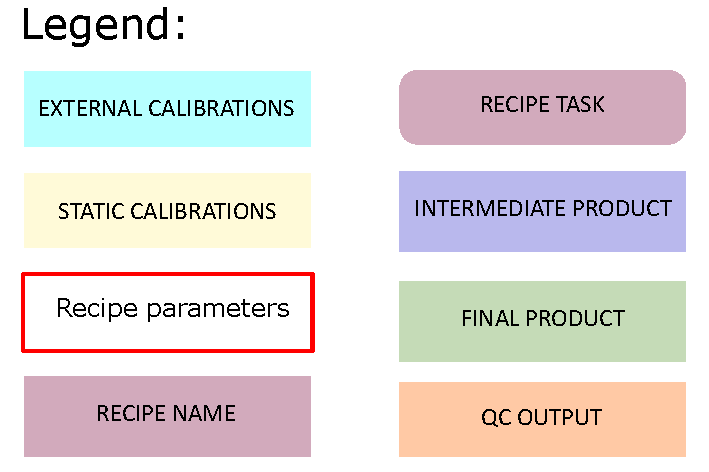
\includegraphics[width=0.4\textheight]{figures/legend.pdf}
  \caption[Legend]{Legend of the coloured boxes in the workflows.}
  \label{Fig:legend}
\end{figure}
\clearpage